\documentclass[]{article}
\usepackage{lmodern}
\usepackage{amssymb,amsmath}
\usepackage{ifxetex,ifluatex}
\usepackage{fixltx2e} % provides \textsubscript
\ifnum 0\ifxetex 1\fi\ifluatex 1\fi=0 % if pdftex
  \usepackage[T1]{fontenc}
  \usepackage[utf8]{inputenc}
\else % if luatex or xelatex
  \ifxetex
    \usepackage{mathspec}
    \usepackage{xltxtra,xunicode}
  \else
    \usepackage{fontspec}
  \fi
  \defaultfontfeatures{Mapping=tex-text,Scale=MatchLowercase}
  \newcommand{\euro}{€}
\fi
% use upquote if available, for straight quotes in verbatim environments
\IfFileExists{upquote.sty}{\usepackage{upquote}}{}
% use microtype if available
\IfFileExists{microtype.sty}{%
\usepackage{microtype}
\UseMicrotypeSet[protrusion]{basicmath} % disable protrusion for tt fonts
}{}
\usepackage[margin=1in]{geometry}
\usepackage{color}
\usepackage{fancyvrb}
\newcommand{\VerbBar}{|}
\newcommand{\VERB}{\Verb[commandchars=\\\{\}]}
\DefineVerbatimEnvironment{Highlighting}{Verbatim}{commandchars=\\\{\}}
% Add ',fontsize=\small' for more characters per line
\newenvironment{Shaded}{}{}
\newcommand{\KeywordTok}[1]{\textcolor[rgb]{0.00,0.44,0.13}{\textbf{{#1}}}}
\newcommand{\DataTypeTok}[1]{\textcolor[rgb]{0.56,0.13,0.00}{{#1}}}
\newcommand{\DecValTok}[1]{\textcolor[rgb]{0.25,0.63,0.44}{{#1}}}
\newcommand{\BaseNTok}[1]{\textcolor[rgb]{0.25,0.63,0.44}{{#1}}}
\newcommand{\FloatTok}[1]{\textcolor[rgb]{0.25,0.63,0.44}{{#1}}}
\newcommand{\CharTok}[1]{\textcolor[rgb]{0.25,0.44,0.63}{{#1}}}
\newcommand{\StringTok}[1]{\textcolor[rgb]{0.25,0.44,0.63}{{#1}}}
\newcommand{\CommentTok}[1]{\textcolor[rgb]{0.38,0.63,0.69}{\textit{{#1}}}}
\newcommand{\OtherTok}[1]{\textcolor[rgb]{0.00,0.44,0.13}{{#1}}}
\newcommand{\AlertTok}[1]{\textcolor[rgb]{1.00,0.00,0.00}{\textbf{{#1}}}}
\newcommand{\FunctionTok}[1]{\textcolor[rgb]{0.02,0.16,0.49}{{#1}}}
\newcommand{\RegionMarkerTok}[1]{{#1}}
\newcommand{\ErrorTok}[1]{\textcolor[rgb]{1.00,0.00,0.00}{\textbf{{#1}}}}
\newcommand{\NormalTok}[1]{{#1}}
\ifxetex
  \usepackage[setpagesize=false, % page size defined by xetex
              unicode=false, % unicode breaks when used with xetex
              xetex]{hyperref}
\else
  \usepackage[unicode=true]{hyperref}
\fi
\hypersetup{breaklinks=true,
            bookmarks=true,
            pdfauthor={},
            pdftitle={Porównanie metod pobierania komórek do przeszczepu},
            colorlinks=true,
            citecolor=blue,
            urlcolor=blue,
            linkcolor=magenta,
            pdfborder={0 0 0}}
\urlstyle{same}  % don't use monospace font for urls
\setlength{\parindent}{0pt}
\setlength{\parskip}{6pt plus 2pt minus 1pt}
\setlength{\emergencystretch}{3em}  % prevent overfull lines
\setcounter{secnumdepth}{0}

%%% Use protect on footnotes to avoid problems with footnotes in titles
\let\rmarkdownfootnote\footnote%
\def\footnote{\protect\rmarkdownfootnote}

%%% Change title format to be more compact
\usepackage{titling}

% Create subtitle command for use in maketitle
\newcommand{\subtitle}[1]{
  \posttitle{
    \begin{center}\large#1\end{center}
    }
}

\setlength{\droptitle}{-2em}
  \title{Porównanie metod pobierania komórek do przeszczepu}
  \pretitle{\vspace{\droptitle}\centering\huge}
  \posttitle{\par}
  \author{}
  \preauthor{}\postauthor{}
  \date{}
  \predate{}\postdate{}

\usepackage{polski}
\usepackage[T1]{fontenc}
\usepackage[utf8]{inputenc} 
%\usepackage[top=1.5cm, bottom=1.5cm, left=0.85cm, right=0.85cm]{geometry}
\usepackage{fancyhdr}
\pagestyle{fancy}
\fancyhead[RO,LE]{\bfseries \small{P. Auguścik, M. Kosiński, B. Sozańska, A. Szewczyk}}
\fancyhead[RE,LO]{\bfseries \small{Biostatystyka, Projekt nr 4}}
\AtBeginDocument{\thispagestyle{fancy}}
\usepackage{rotating}
\usepackage{subfigure}
\usepackage{pdflscape}
\usepackage{amsfonts}
\usepackage{amsmath}
\usepackage{amssymb}
\usepackage{color}
\usepackage{amsthm}
\usepackage{longtable}
\usepackage{wrapfig,booktabs}
\usepackage{tikz}
\usepackage{float}
\usepackage{hyperref} %pakiet do dodawania hiperłącz
\hypersetup{colorlinks=true,
            linkcolor=black,
            citecolor=black,
            urlcolor=black}
%\title{\textbf{\LARGE{Biostatystyka - Projekt zaliczeniowy} }}


\begin{document}

\maketitle


\thispagestyle{fancy}

Głownym celem było porównanie dwóch metod pobierania komórek do
przeszczepu. Tradycyjna, bardziej inwazyjna polega na pobraniu z kości
miednicy, oraz mniej inwazyjna, czyli pobieranie szpiku z krwi
obwodowej. Analizie poddano pacjentów dotkniętych dwoma typami
białaczki: ostrą i przewlekłą. Dla pacjentów mierzono czas do
wystąpienia pierwszego ze zdarzeń: czas do nawrotu choroby, czas do
pojawienia się symptomów przewlekłego odrzutu przeszczepu oraz czas
przeżycia (do zgonu).

\vspace{10pt}

\textbf{Sub-dystrybuanty}

Chcąc zbadać wpływ poszczególnych zmiennych dyskretnych na czas do
wystąpienia zdarzenia sporządzono wykresy sub-dystrybuant. Dla
poszczególnych typów zdarzeń oszacowania sub-dystrybuant wyglądają
następująco:

\begin{itemize}
\itemsep1pt\parskip0pt\parsep0pt
\item
  Dla metody pobierania komórek do przeszczepu
\end{itemize}

\vspace{-22pt}

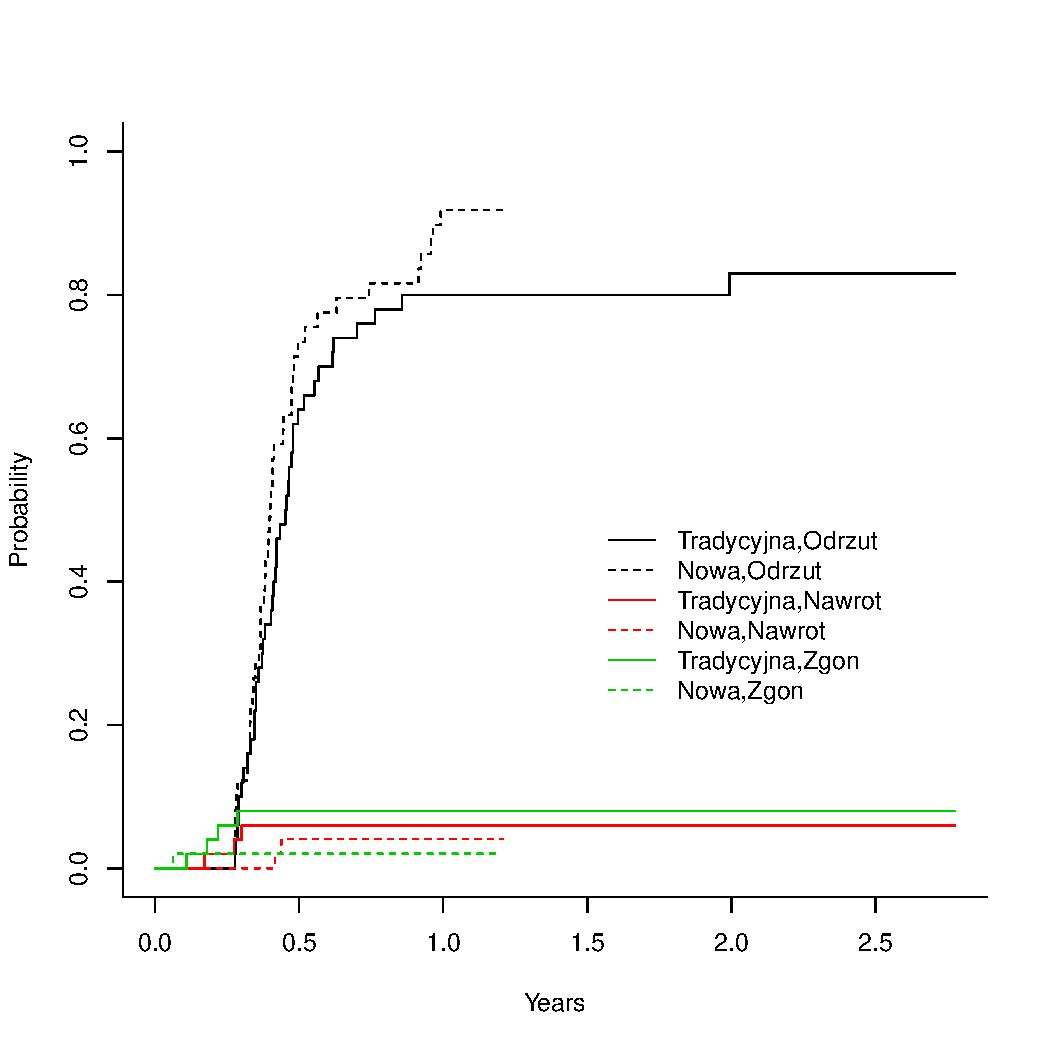
\includegraphics[width=16cm,height=7.2cm]{plot1.pdf}

\begin{itemize}
\itemsep1pt\parskip0pt\parsep0pt
\item
  Dla typu białaczki
\end{itemize}

\vspace{-22pt}

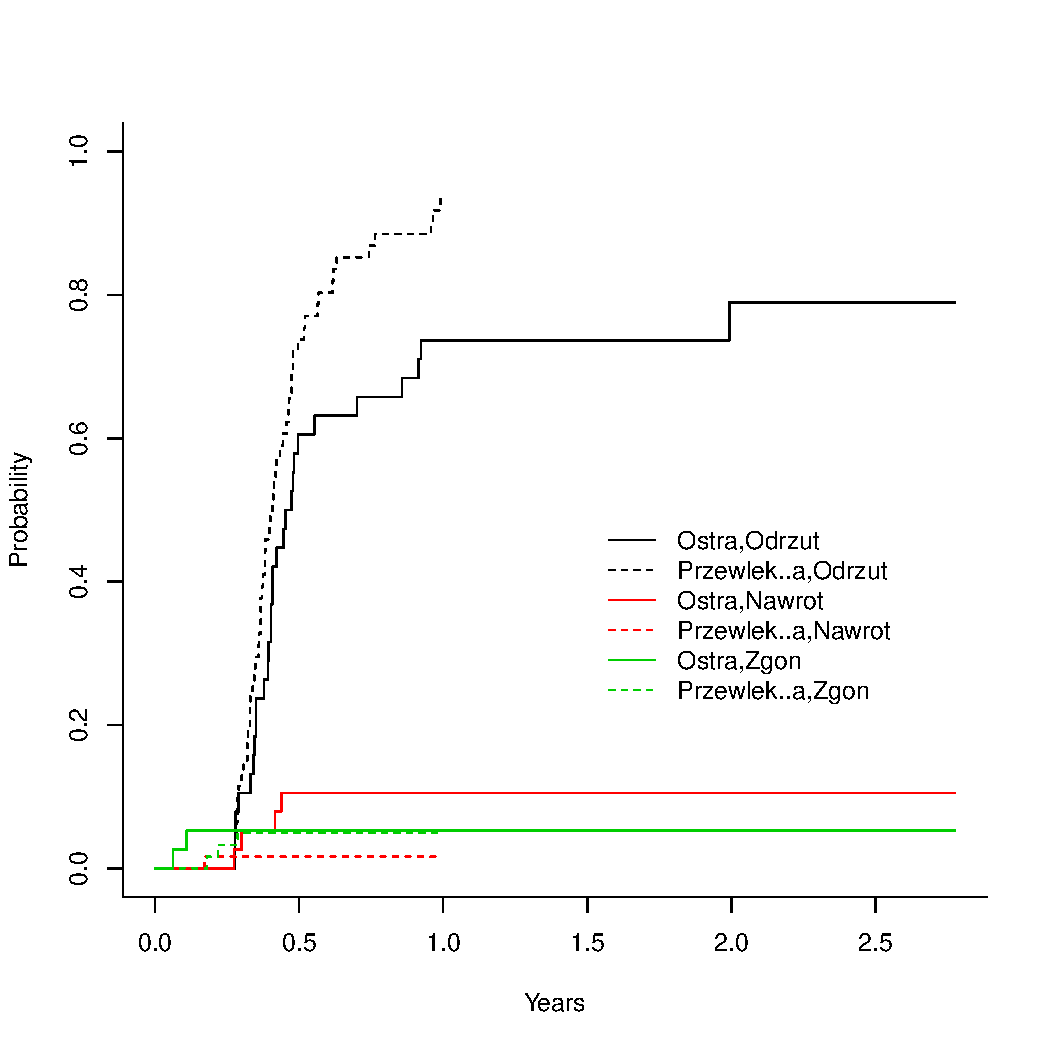
\includegraphics[width=16cm,height=8.2cm]{plot2.pdf} \newpage

\textbf{Test Graya}

Formalnie przy użyciu testu Graya można sprawdzić czy różnice w
oszacowanych sub-dystrybuantach są istotne statystycznie w podziale na
podgrupy ze względu na zmienne:

\begin{itemize}
\itemsep1pt\parskip0pt\parsep0pt
\item
  Dla metod pobierania komórek do przeszczepu:
\end{itemize}

\begin{verbatim}
       stat        pv df
1 2.0192451 0.1553163  1
2 0.2114488 0.6456342  1
3 1.7635527 0.1841820  1
\end{verbatim}

\begin{itemize}
\itemsep1pt\parskip0pt\parsep0pt
\item
  Dla typu białaczki:
\end{itemize}

\begin{verbatim}
        stat         pv df
1 5.34343189 0.02080048  1
2 3.71906498 0.05379449  1
3 0.01090047 0.91684770  1
\end{verbatim}

Z podsumowania testów widać, że zachodzą jedynie statystycznie istotne
różnice w oszacowanych sub-dystrybuantach dla typu białaczki dla
pierwszego typu zdarzenia, czyli odrzutu, na zakładanym poziomie
istotności $\alpha=0.05$ (wartość krytyczna testu jest równa
$0.02080048$). Można to również zaobserwować na poniższym wykresie
prezentującym sub-dystrybuanty dla typu zdarzenia jakim jest odrzut, z
podziałem na typ białaczki.

\begin{center}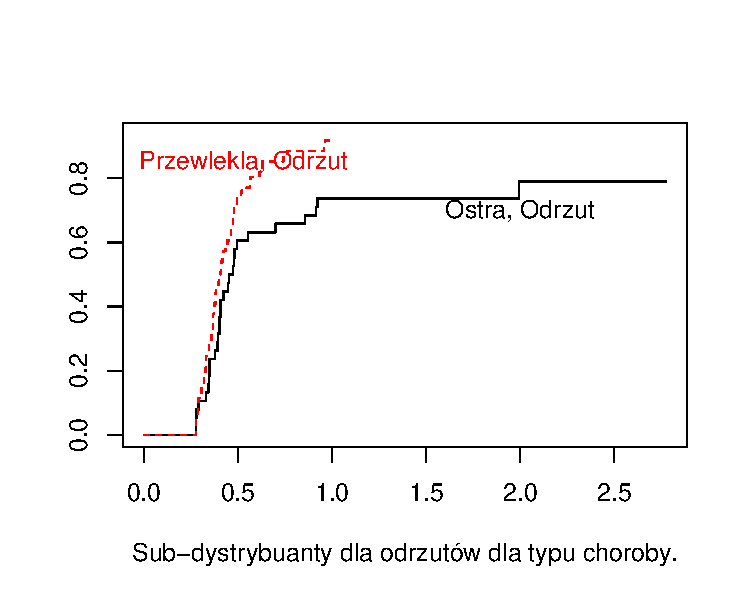
\includegraphics{figure/beamer-unnamed-chunk-8-1} \end{center}

Widać, że oszacowana sub-dystrybuanta dla \emph{ostrej} białaczki leży
poniżej oszacowanej sub-dystrybuanty dla \emph{przewlekłego} typu tej
choroby, co oznacza, że pacjenci z \emph{ostrą} białaczką mają dłuższe
czasy do zdarzenia jakim jest odrzut przeszczepu.

\newpage
\textbf{Modele proporcjonalnych hazardów}

Dla danych dotyczących wieku pacjenta, typu białaczki i metody pobrania
komórek do przeszczepu dopasowujemy model PH dla funkcji hazardów
`specyficznych dla typów'. Podsumownia modeli dla typów zdarzeń: odrzut,
nawrót, zgon, zaprezentowano poniżej.

\begin{verbatim}
Call:
coxph(formula = Surv(first_t, first_e == 1) ~ diag + trt + age, 
    data = dane.red)

        coef exp(coef) se(coef)      z     p
diag  0.4712      1.60   0.2368  1.990 0.047
trt   0.0602      1.06   0.2201  0.274 0.780
age  -0.0104      0.99   0.0103 -1.006 0.310
\end{verbatim}

\begin{verbatim}
Call:
coxph(formula = Surv(first_t, first_e == 2) ~ diag + trt + age, 
    data = dane.red)

        coef exp(coef) se(coef)       z     p
diag -1.9448     0.143   1.1361 -1.7118 0.087
trt  -0.0800     0.923   0.9689 -0.0825 0.930
age  -0.0484     0.953   0.0433 -1.1182 0.260
\end{verbatim}

\begin{verbatim}
Call:
coxph(formula = Surv(first_t, first_e == 3) ~ diag + trt + age, 
    data = dane.red)

        coef exp(coef) se(coef)      z     p
diag -0.3965     0.673   0.9735 -0.407 0.680
trt  -1.5046     0.222   1.1522 -1.306 0.190
age   0.0973     1.102   0.0588  1.655 0.098
\end{verbatim}

Na badanym, zakładanym poziomie istotności $\alpha=0.05$, statystycznie
istotnie różny od 0 jest współczynnik przy zmiennej \textsf{diag}
odpowiadającej typowi białaczki w modelu dla zdarzenia jakim jest
wystąpienie symptomów odrzutu przeszczepu -- wartość krytyczna testu
wyniosła $0.047<0.05$. Białaczka przewlekła ma o 60\% większy hazard
`specyficzny dla typu' zdarzenia jakim jest odrzut. Dla pozostałych
zmiennych dla tego typu zdarzenia oraz wszystkich zmiennych
\text{w pozostałych} typach zdarzenia, nie ma statystycznie istotnych
podstaw, aby odrzucić hipotezę zerową mówiącą o tym, że współczynnik w
modelu jest równy 0.

Sporządzono również model hazardu sub-dystrybuanty, którego podsumowanie
wygląda następująco:

\begin{verbatim}
convergence:  TRUE 
coefficients:
    diag      trt      age 
 0.53950  0.31860 -0.01188 
standard errors:
[1] 0.228400 0.207900 0.009176
two-sided p-values:
 diag   trt   age 
0.018 0.130 0.200 
\end{verbatim}

\begin{verbatim}
convergence:  TRUE 
coefficients:
    diag      trt      age 
-1.91300 -0.12670 -0.04486 
standard errors:
[1] 1.2150 0.9466 0.0337
two-sided p-values:
diag  trt  age 
0.12 0.89 0.18 
\end{verbatim}

\begin{verbatim}
convergence:  TRUE 
coefficients:
    diag      trt      age 
-0.38580 -1.50400  0.09887 
standard errors:
[1] 0.7938 1.1230 0.0513
two-sided p-values:
 diag   trt   age 
0.630 0.180 0.054 
\end{verbatim}

Podobnie w modelu hazardu dla sub-dystrybuanty, jedyną zmienną istotnie
statystycznie różną od 0 jest zmienna \textsf{diag} dla modelu dla typu
zdarzenia jakim jest pojawienie się symptomów odrzutu przeszczepu,
której wartość krytyczna testu $0.018<0.05$ jest mniejsza od zakładanego
poziomu istotności. Hazard dla sub-dystrybuanty dla pacjenta z
przewlekłą białaczką jest o 71,5 \% większy niż dla pacjenta z ostrą
białaczką. Dla pozostałych zmiennych w tym modelu i dla wszystkich
zmiennych w pozostałych modelach dla tych zmiennych nie ma statystycznie
istotnych podstaw by odrzucić hipotezy zerowe o tym, że współczynniki są
równe 0.

\vspace{10pt}

\textbf{Podsumowanie}

Zarówno modele dla funkcji hazardu `specyficznych dla typu' jak i modele
dla hazardów sub-dystrybuanty dały podobne wyniki. Jedynym istotnym
współczynnikiem jest współczynnik przy zmiennej \textsf{diag}
odpowiadającej typowi białaczki w modelach dla zdarzenia jakim jest
wystąpienie symptomów odrzutu przeszczepu. \text{Dla pozostałych}
zmiennych dla tego typu zdarzenia oraz wszystkich zmiennych w
pozostałych typach zdarzeń oba podejścia modelowe nie dają podstaw do
odrzucenia hipotezy o tym, że współczynniki przy zmiennej są równe 0. Na
tej podstawie stwierdzamy, że jedyną istotną zmienną jest typ białaczki,
gdy rozpatrujemy zdarzenie odrzutu przeszczepu. Zmienna ta oraz
pozostałe, w modelach dla zdarzeń jakimi są nawrót oraz zgon, mogły
okazać się nieistotne statystycznie z powodu zbyt małej liczby zdarzeń
tych typów. Zmienna określająca sposób pobierania komórek do przeszczepu
w obu modelach jest nieistotna statystycznie, zatem nie wpływa to
istotnie na czas do wystąpienia poszczególnych badanych zdarzeń. Obie
metody pod tym względem są porównywalne, lecz biorąc pod uwagę
inwazyjność metod, nasuwa się wniosek, że pobieranie szpiku z krwi
obwodowej daje pacjentowi większy komfort leczenia w porównaniu do
tradycyjnej metody pobierania komórek z kości miednicy.

\newpage
\small
\textbf{Kody}

\begin{Shaded}
\begin{Highlighting}[]
\KeywordTok{library}\NormalTok{(survival)}
\NormalTok{dane <-}\StringTok{ }\KeywordTok{read.csv}\NormalTok{(}\StringTok{"bmt.csv"}\NormalTok{)}
\NormalTok{dane.red <-}\StringTok{ }\KeywordTok{data.frame}\NormalTok{(dane, }\DataTypeTok{event=}\KeywordTok{ifelse}\NormalTok{(dane$first_e==}\DecValTok{0}\NormalTok{,}\DecValTok{0}\NormalTok{,}\DecValTok{1}\NormalTok{),}
                       \DataTypeTok{odrzut=}\KeywordTok{ifelse}\NormalTok{(dane$first_e==}\DecValTok{1}\NormalTok{,}\DecValTok{1}\NormalTok{,}\DecValTok{0}\NormalTok{), }
                       \DataTypeTok{nawrot=}\KeywordTok{ifelse}\NormalTok{(dane$first_e==}\DecValTok{2}\NormalTok{,}\DecValTok{1}\NormalTok{,}\DecValTok{0}\NormalTok{),}
                       \DataTypeTok{zgon=}\KeywordTok{ifelse}\NormalTok{(dane$first_e==}\DecValTok{3}\NormalTok{,}\DecValTok{1}\NormalTok{,}\DecValTok{0}\NormalTok{))}
\KeywordTok{library}\NormalTok{(cmprsk)}
\KeywordTok{attach}\NormalTok{(dane)}
\NormalTok{ci.trt <-}\StringTok{ }\KeywordTok{cuminc}\NormalTok{(first_t, first_e, }\DataTypeTok{group=}\NormalTok{trt) }
\KeywordTok{plot}\NormalTok{(ci.trt, }\DataTypeTok{curvlab=}\KeywordTok{c}\NormalTok{(}\StringTok{"Tradycyjna,Odrzut"}\NormalTok{, }
                       \StringTok{"Nowa,Odrzut"}\NormalTok{,}
                       \StringTok{"Tradycyjna,Nawrot"}\NormalTok{,}
                       \StringTok{"Nowa,Nawrot"}\NormalTok{,}
                       \StringTok{"Tradycyjna,Zgon"}\NormalTok{,}
                       \StringTok{"Nowa,Zgon"}\NormalTok{), }\DataTypeTok{col=}\KeywordTok{c}\NormalTok{(}\DecValTok{1}\NormalTok{,}\DecValTok{1}\NormalTok{,}\DecValTok{2}\NormalTok{,}\DecValTok{2}\NormalTok{,}\DecValTok{3}\NormalTok{,}\DecValTok{3}\NormalTok{), }\DataTypeTok{wh=}\KeywordTok{c}\NormalTok{(}\FloatTok{1.5}\NormalTok{,}\FloatTok{0.5}\NormalTok{),}
     \DataTypeTok{lty =} \KeywordTok{c}\NormalTok{(}\DecValTok{1}\NormalTok{,}\DecValTok{2}\NormalTok{,}\DecValTok{1}\NormalTok{,}\DecValTok{2}\NormalTok{,}\DecValTok{1}\NormalTok{,}\DecValTok{2}\NormalTok{))}
\NormalTok{ci.diag <-}\StringTok{ }\KeywordTok{cuminc}\NormalTok{(first_t, first_e, }\DataTypeTok{group=}\NormalTok{diag)}
\KeywordTok{plot}\NormalTok{(ci.diag, }\DataTypeTok{curvlab=}\KeywordTok{c}\NormalTok{(}\StringTok{"Ostra,Odrzut"}\NormalTok{, }
                       \StringTok{"Przewlekla,Odrzut"}\NormalTok{,}
                       \StringTok{"Ostra,Nawrot"}\NormalTok{,}
                       \StringTok{"Przewlekla,Nawrot"}\NormalTok{,}
                       \StringTok{"Ostra,Zgon"}\NormalTok{,}
                       \StringTok{"Przewlekla,Zgon"}\NormalTok{),}
     \DataTypeTok{col=}\KeywordTok{c}\NormalTok{(}\DecValTok{1}\NormalTok{,}\DecValTok{1}\NormalTok{,}\DecValTok{2}\NormalTok{,}\DecValTok{2}\NormalTok{,}\DecValTok{3}\NormalTok{,}\DecValTok{3}\NormalTok{), }\DataTypeTok{lty =} \KeywordTok{c}\NormalTok{(}\DecValTok{1}\NormalTok{,}\DecValTok{2}\NormalTok{,}\DecValTok{1}\NormalTok{,}\DecValTok{2}\NormalTok{,}\DecValTok{1}\NormalTok{,}\DecValTok{2}\NormalTok{), }\DataTypeTok{wh =} \KeywordTok{c}\NormalTok{(}\FloatTok{1.5}\NormalTok{,}\FloatTok{0.5}\NormalTok{))}
\KeywordTok{library}\NormalTok{(cmprsk)}
\KeywordTok{attach}\NormalTok{(dane.red)}
\NormalTok{ci.trt <-}\StringTok{ }\KeywordTok{cuminc}\NormalTok{(first_t, first_e, }\DataTypeTok{group=}\NormalTok{trt)}
\NormalTok{ci.trt$Tests}
\NormalTok{ci.diag <-}\StringTok{ }\KeywordTok{cuminc}\NormalTok{(first_t, first_e, }\DataTypeTok{group=}\NormalTok{diag)}
\NormalTok{ci.diag$Tests}
\NormalTok{ci.sfit <-}\StringTok{ }\KeywordTok{survfit}\NormalTok{(}\KeywordTok{Surv}\NormalTok{(first_t, event)~diag, }\DataTypeTok{etype=}\NormalTok{first_e, }\DataTypeTok{data=}\NormalTok{dane.red)}
\KeywordTok{plot}\NormalTok{(ci.sfit, }\DataTypeTok{lty=}\KeywordTok{c}\NormalTok{(}\DecValTok{1}\NormalTok{,}\DecValTok{0}\NormalTok{,}\DecValTok{0}\NormalTok{,}\DecValTok{2}\NormalTok{,}\DecValTok{0}\NormalTok{,}\DecValTok{0}\NormalTok{), }\DataTypeTok{col=}\DecValTok{1}\NormalTok{:}\DecValTok{2}\NormalTok{, }\DataTypeTok{mark.time=}\NormalTok{F, }\DataTypeTok{conf.int=}\NormalTok{F, }\DataTypeTok{xscale=}\DecValTok{1}\NormalTok{, }
     \DataTypeTok{xlab=}\StringTok{"Sub-dystrybuanty dla odrzutów dla typu choroby."}\NormalTok{)}
\KeywordTok{text}\NormalTok{(}\DecValTok{2}\NormalTok{, }\FloatTok{0.7}\NormalTok{,}\StringTok{"Ostra, Odrzut"}\NormalTok{, }\DataTypeTok{col=}\DecValTok{1}\NormalTok{)}
\KeywordTok{text}\NormalTok{(}\FloatTok{0.53}\NormalTok{, }\FloatTok{0.85}\NormalTok{,}\StringTok{"Przewlekla, Odrzut"}\NormalTok{, }\DataTypeTok{col=}\DecValTok{2}\NormalTok{)}
\KeywordTok{print}\NormalTok{(coxph.odrzut <-}\StringTok{ }
\StringTok{          }\KeywordTok{coxph}\NormalTok{(}\KeywordTok{Surv}\NormalTok{(first_t, first_e ==}\StringTok{ }\DecValTok{1}\NormalTok{) ~}\StringTok{ }\NormalTok{diag+trt+age,}
                            \DataTypeTok{data =} \NormalTok{dane.red))}
\KeywordTok{print}\NormalTok{(coxph.nawrot <-}\StringTok{ }
\StringTok{          }\KeywordTok{coxph}\NormalTok{(}\KeywordTok{Surv}\NormalTok{(first_t, first_e ==}\StringTok{ }\DecValTok{2}\NormalTok{) ~}\StringTok{ }\NormalTok{diag+trt+age,}
                          \DataTypeTok{data =} \NormalTok{dane.red))}
\KeywordTok{print}\NormalTok{(coxph.zgon <-}\StringTok{ }
\StringTok{          }\KeywordTok{coxph}\NormalTok{(}\KeywordTok{Surv}\NormalTok{(first_t, first_e ==}\StringTok{ }\DecValTok{3}\NormalTok{) ~}\StringTok{ }\NormalTok{diag+trt+age,}
                          \DataTypeTok{data =} \NormalTok{dane.red))}
\KeywordTok{model.matrix}\NormalTok{(~}\StringTok{ }\NormalTok{diag+trt+age)[,-}\DecValTok{1}\NormalTok{] ->}\StringTok{ }\NormalTok{m.dane.red}
\NormalTok{(mod.odrzut <-}\StringTok{ }\KeywordTok{crr}\NormalTok{(}\DataTypeTok{ftime=}\NormalTok{first_t, }\DataTypeTok{fstatus=}\NormalTok{first_e,}
                        \DataTypeTok{cov1=} \NormalTok{m.dane.red,}
                        \CommentTok{#cov2 = trt,}
                        \DataTypeTok{failcode=}\DecValTok{1}\NormalTok{))}
\NormalTok{(mod.nawrot <-}\StringTok{ }\KeywordTok{crr}\NormalTok{(}\DataTypeTok{ftime=}\NormalTok{first_t, }\DataTypeTok{fstatus=}\NormalTok{first_e,}
                          \DataTypeTok{cov1=} \NormalTok{m.dane.red,}
                          \CommentTok{#cov2 = trt,}
                          \DataTypeTok{failcode=}\DecValTok{2}\NormalTok{))}
\NormalTok{(mod.zgon <-}\StringTok{ }\KeywordTok{crr}\NormalTok{(}\DataTypeTok{ftime=}\NormalTok{first_t, }\DataTypeTok{fstatus=}\NormalTok{first_e,}
                          \DataTypeTok{cov1=} \NormalTok{m.dane.red,}
                          \CommentTok{#cov2 = trt,}
                          \DataTypeTok{failcode=}\DecValTok{3}\NormalTok{))}
\end{Highlighting}
\end{Shaded}

\end{document}
